\subsection{JSON}

A continuación, queremos crear de nuevo una tabla que contenga todos los datos de los partidos (países, torneos, ediciones, partidos, sets y jugadores). Concretamente, está vez debe resolver de forma eficiente las consultas Q2 y Q4. Para mantener orden en nuestra bae de datos, crearemos un nueva esquema \texttt{agregadosJSON} para alojar esta nueva tabla. \\

PostgreSQL proporciona un tipo de datos ``json'' y un conjunto de funciones y operadores que permiten tanto generar documentos JSON a partir de datos relacionales como consultar partes de un documento JSON. Además del tipo ``json'', también se proporciona un tipo más eficiente ``jsonb'', que almacena los documentos en formato binario. Para resolver de forma eficiente las consultas deseadas, nuestra tabla deberá estar orientada a los jugadores, es decir, una tupla para cada jugador con todos sus datos y los partidos que ha jugado. \\

En el caso de JSON (usaremos JSONB), tenemos objetos JSON y agregados de objetos JSON. La creación del esquema de la tabla y la inserción de los datos se realiza mediante la misma consulta, que explicamos a continuación.  \\


Comenzaremos con la tabla \texttt{jugador}, y haremos un \textit{left join} con la tabla \texttt{pais} para obtener los datos del país del jugador. El motivo del \textit{left join} en lugar de un \textit{inner join} lo comentamos en la sección de agregados de tipos compuestos. En el \texttt{where} realizamos un paso crítico para la eficiencia de la consulta: filtramos los jugadores que han participado en algún partido. Para ello, seleccionamos los jugadores cuyo id está en la lista de perdedores o ganadores de algún partido. Debemos hacer esto ya que, de los 60 mil jugadores existentes en la base de datos, unos 58 mil no ganaron ni perdieron ningún partido (según los datos recogidos en nuestra base de datos relacional). \\

Con esto tenemos la tuplas de los partidos jugadores que han participado en algún partido. Al obtener la proyección, haremos que cada tupla tenga los siguientes atributos: 
\begin{itemize}
\item \texttt{jugador}: objeto jsonb con los datos del jugador: id, nombre, apellido, diestro, fecha de nacimiento y altura.
\item \texttt{pais}: objeto jsonb con los datos del país del jugador: código ISO2, código ISO3, código IOC y nombre.
\item \texttt{partidos\_ganados}: agregación de objetos jsonb con los datos de los partidos ganados por el jugador. Cada objeto jsonb será un partido concreto y contendrá los datos del torneo, la fecha, la ronda, el desenlace, el número de partido, el rival, los sets y las estadísticas del jugador y las del rival. \\

La agregación de objetos jsonb se hace mediante subconsultas, por lo que debemos pararnos a explicar la construcción de este agregado más en detalle. Para esta subconsulta partimos de la tabla \texttt{partido}, que denotaremos por el alias \texttt{pg} al estar tratando con los partidos ganados, y realizamos un \textit{left join} con la tabla \texttt{edicion\_torneo} mediante los atributos que definen la FK de la tabla \texttt{partido} y la PK de la tabla \texttt{edicion\_torneo}. A continuación, realizamos un \textit{left join} con la tabla \texttt{torneo} mediante los atributos que definen la FK de la tabla \texttt{edicion\_torneo} y la PK de la tabla \texttt{torneo}. Finalmente, hacemos otro \textit{left join} con la tabla \texttt{pais} mediante el codigo ISO2. Seleccionamos solo los partidos ganados por el jugador que estamos tratando y construimos un objeto jsonb con los datos del torneo, la fecha, la ronda, el desenlace, el número de partido, el rival, los sets y las estadísticas del jugador y las del rival. \\

De estos atributos, \texttt{fecha}, \texttt{ronda}, \texttt{desenlace}, \texttt{num\_partido} y \texttt{perdedor} son directamente obtenidos de la tabla \texttt{partido pg}. Además, \texttt{torneo} es simplemente un objeto jsonb con los datos relativos asa edicion del torneo: nombre, pais (que será un objeto jsonb con los atributos del país que se reflejan en la tabla relacional de \texttt{pais}), fecha, superficie, tamaño y nivel. Las estadísticas de el jugador y del rival son también objetos jsonb que toman los datos estadísticos de la tabla \texttt{partido pg}. \\

Por último, los sets son un agregado de objetos jsonb que se construye mediante una subconsulta que selecciona los sets de un partido concreto. Cada objeto jsonb de este agregado contiene el número de set, los juegos ganados por el jugador, los juegos ganados por el rival y los puntos del tiebreak en caso de que se haya llegado a este. Para hacer la subconsulta descrita nos centramos en la tabla \texttt{sets\_partido}. La unimos con condiciones de \textit{join} a \texttt{partido}, igualando los atributos que componen la clave foránea de \texttt{sets\_partido} con los atributos que componen la clave primaria de \texttt{partido}, seleccionando así solo los sets del partido que estamos tratando. 
\item \texttt{partidos\_perdidos}: este agregado de objetos jsonb lo obtenemos de forma completamente análoga a \texttt{partidos\_ganados}, pero con los partidos perdidos por el jugador.
\end{itemize}


\begin{minted}[frame=single, fontsize=\footnotesize]{sql}
create table tenisjson as
select 
	-- columna 'jugador' como objeto json
	jsonb_build_object(
		'id', j.id, 
		'nombre', j.nombre, 
		'apellido', j.apellido, 
		'diestro', j.diestro, 
		'fecha_nacimiento', j.fecha_nacimiento, 
		'altura', j.altura
	) as jugador,
  -- columna 'pais' como objeto json
	jsonb_build_object(
		'codigo_iso2', p.codigo_iso2, 
		'codigo_iso3', p.codigo_iso3, 
		'codigo_ioc', p.codigo_ioc, 
		'nombre', p.nombre
	) as pais,
  -- columna 'partidos_ganados' como agregado json
	(select jsonb_agg(jsonb_build_object(
		'torneo', jsonb_build_object(
			'nombre', t.nombre, 
			'pais', jsonb_build_object(
				'codigo_iso2', pa.codigo_iso2, 
				'codigo_iso3', pa.codigo_iso3, 
				'codigo_ioc', pa.codigo_ioc, 
				'nombre', pa.nombre), 
			'fecha', et.fecha, 
			'superficie', et.superficie, 
			'tamano', et.tamano, 
			'nivel', et.nivel), 
		'fecha', pg.fecha, 
		'ronda', pg.ronda, 
		'desenlace', pg.desenlace, 
		'num_partido', pg.num_partido, 
		'rival', pg.perdedor, 
		'sets', (select jsonb_agg(
			jsonb_build_object(
				'num_set', sp.num_set, 
				'juegos_ganador', sp.juegos_ganador, 
				'juegos_perdedor', sp.juegos_perdedor, 
				'puntos_tiebreak_perdedor', sp.puntos_tiebreak_perdedor
			)
		) 
		from sets_partido sp 
		where sp.torneo = pg.torneo 
			and sp.fecha = pg.fecha 
			and sp.num_partido = pg.num_partido), 
		'stats', jsonb_build_object(
			'num_aces', pg.num_aces_ganador, 
			'num_dob_faltas', pg.num_dob_faltas_ganador, 
			'num_puntos_servidos', pg.num_ptos_servidos_ganador, 
			'num_primeros_servicios', pg.num_primeros_servicios_ganador, 
			'num_primeros_servicios_ganados', pg.num_primeros_servicios_ganados_ganador, 
			'num_segundos_servicios_ganados', pg.num_segundos_servicios_ganados_ganador, 
			'num_juegos_servidos', pg.num_juegos_servidos_ganador, 
			'num_break_salvados', pg.num_break_salvados_ganador, 
			'num_break_afrontados', pg.num_break_afrontados_ganador
		), 
		'stats_rival', jsonb_build_object(
			'num_aces', pg.num_aces_perdedor, 
			'num_dob_faltas', pg.num_dob_faltas_perdedor, 
			'num_puntos_servidos', pg.num_ptos_servidos_perdedor, 
			'num_primeros_servicios', pg.num_primeros_servicios_perdedor, 
			'num_primeros_servicios_ganados', pg.num_primeros_servicios_ganados_perdedor, 
			'num_segundos_servicios_ganados', pg.num_segundos_servicios_ganados_perdedor, 
			'num_juegos_servidos', pg.num_juegos_servidos_perdedor, 
			'num_break_salvados', pg.num_break_salvados_perdedor, 
			'num_break_afrontados', pg.num_break_afrontados_perdedor
		)
	)) 
	from public.partido pg 
		left join public.edicion_torneo et on pg.torneo = et.torneo and pg.fecha = et.fecha 
		left join public.torneo t on et.torneo = t.id 
		left join public.pais pa on t.pais = pa.codigo_iso2
	where pg.ganador = j.id) as partidos_ganados,
   -- columna 'partidos_perdidos' como json
	(select jsonb_agg(jsonb_build_object(
		'torneo', jsonb_build_object(
			'nombre', t.nombre, 
			'pais', jsonb_build_object(
				'codigo_iso2', pa.codigo_iso2,
				'codigo_iso3', pa.codigo_iso3,
				'codigo_ioc', pa.codigo_ioc,
				'nombre', pa.nombre
			),
			'fecha', et.fecha,
			'superficie', et.superficie,
			'tamano', et.tamano,
			'nivel', et.nivel
		),
		'fecha', pp.fecha,
		'ronda', pp.ronda,
		'desenlace', pp.desenlace,
		'num_partido', pp.num_partido,
		'rival', pp.ganador,
		'sets', (select jsonb_agg(
			jsonb_build_object(
				'num_set', sp.num_set,
				'juegos_ganador', sp.juegos_ganador,
				'juegos_perdedor', sp.juegos_perdedor,
				'puntos_tiebreak_perdedor', sp.puntos_tiebreak_perdedor
			)
		) 
		from sets_partido sp 
		where sp.torneo = pp.torneo 
			and sp.fecha = pp.fecha 
			and sp.num_partido = pp.num_partido),
		'stats', jsonb_build_object(
			'num_aces', pp.num_aces_perdedor,
			'num_dob_faltas', pp.num_dob_faltas_perdedor,
			'num_puntos_servidos', pp.num_ptos_servidos_perdedor,
			'num_primeros_servicios', pp.num_primeros_servicios_perdedor,
			'num_primeros_servicios_ganados', pp.num_primeros_servicios_ganados_perdedor,
			'num_segundos_servicios_ganados', pp.num_segundos_servicios_ganados_perdedor,
			'num_juegos_servidos', pp.num_juegos_servidos_perdedor,
			'num_break_salvados', pp.num_break_salvados_perdedor,
			'num_break_afrontados', pp.num_break_afrontados_perdedor
		),
		'stats_rival', jsonb_build_object(
			'num_aces', pp.num_aces_ganador,
			'num_dob_faltas', pp.num_dob_faltas_ganador,
			'num_puntos_servidos', pp.num_ptos_servidos_ganador,
			'num_primeros_servicios', pp.num_primeros_servicios_ganador,
			'num_primeros_servicios_ganados', pp.num_primeros_servicios_ganados_ganador,
			'num_segundos_servicios_ganados', pp.num_segundos_servicios_ganados_ganador,
			'num_juegos_servidos', pp.num_juegos_servidos_ganador,
			'num_break_salvados', pp.num_break_salvados_ganador,
			'num_break_afrontados', pp.num_break_afrontados_ganador
		)
	)) 
	from public.partido pp
		left join public.edicion_torneo et on pp.torneo = et.torneo and pp.fecha = et.fecha
		left join public.torneo t on et.torneo = t.id
		left join public.pais pa on t.pais = pa.codigo_iso2
	where pp.perdedor = j.id) as partidos_perdidos
from public.jugador j
	left join public.pais p on j.pais = p.codigo_iso2
where j.id in (select perdedor from public.partido)
	or j.id in (select ganador from public.partido)
\end{minted}

\noindent Antes de comenzar con las consultas, comentamos los aspectos clave:
\begin{itemize}
\item Para acceder a un valor como un objeto jsonb completo, usamos la notación ->. 
\item Para acceder a un valor como un texto, usamos la notación ->>.
\item Para acceder a elementos de un array jsonb, debemos usar la función \texttt{jsonb\_array\_elements(nombre\_array)}. Esto extrae los elementos y los asigna a registros independientes. Esto es similar a la función \texttt{unnest} que usamos en los arrays de PostgreSQL y, del mismo modo, se puede asignar un alias a cada elemento del array.
\end{itemize}

Así, por ejemplo, para acceder al nombre de un torneo, con la estrucura que creamos, debemos desagregar al agregado jsonb `partidos ganados' con \texttt{jsonb\_array\_elements(partidos\_ganados)} y acceder al campo `torneo' con -> (ya que es un objeto jsonb) y al campo `nombre' con ->>. Así, si previamente asignamos a \texttt{jsonb\_array\_elements(partidos\_ganados)} el alias \texttt{partidos(pg)}, cada elemento del array se denotará por ``pg'', y podremos acceder al nombre del torneo como \texttt{pg} -> \texttt{`torneo'} ->> \texttt{`nombre'}. 

\subsubsection{Muestra todos los ganadores del torneo ``Wimbledon'' (Nombre apellidos y año). Ordena el resultado por año.}

El ejemplo anterior nos resulta útil para resolver esta consulta (curiosamente usa uno de los atributos que necesitamos\dots). Para esta consulta partimos del producto cartesiano de la tabla \texttt{tenisjson} con la función \texttt{jsonb\_array\_elements(partidos\_ganados)} para extraer los elementos jsonb de partidos ganados. Con esto, estamos generando tuplas que no nos son de utilidad para la consulta, así que debemos hacer una selección en el \texttt{where} para quedarnos solo con los partidos finales de Wimbledon. Para ello, seleccionamos los partidos finales (a ronda accedemos desde ``pg'' con ->>, ya que queremos el resultado como texto) cuyo torneo tenga nombre ``Wimbledon'' (aquí tenemos el ejemplo anterior). A continuación, seleccionamos el nombre y apellido del jugador y el año del torneo como atributos de texto. Aquí hay una sutileza a tener en cuenta: como estamos obteniendo la fecha en formato texto al usar ->>, debemos convertirla a tipo \texttt{date} con \texttt{::date} antes de usar el \texttt{extract(year \dots)} que venimos usando durante todo el trabajo. Finalmente, ordenamos el resultado por año. La consulta se muestra a continuación, y el resultado es el esperado (figura \ref{fig:q1_json})

\begin{minted}[frame=single, fontsize=\footnotesize]{sql}
select tj.jugador ->> 'nombre' as nombre, 
    tj.jugador ->> 'apellido' as apellido, 
    extract(year from (pg ->> 'fecha')::date) as ano
from tenisjson tj, jsonb_array_elements(partidos_ganados) as partidos(pg)
where pg ->> 'ronda' = 'F' 
    and pg -> 'torneo' ->> 'nombre' = 'Wimbledon'
order by ano
\end{minted}

\begin{figure}[H]
\centering
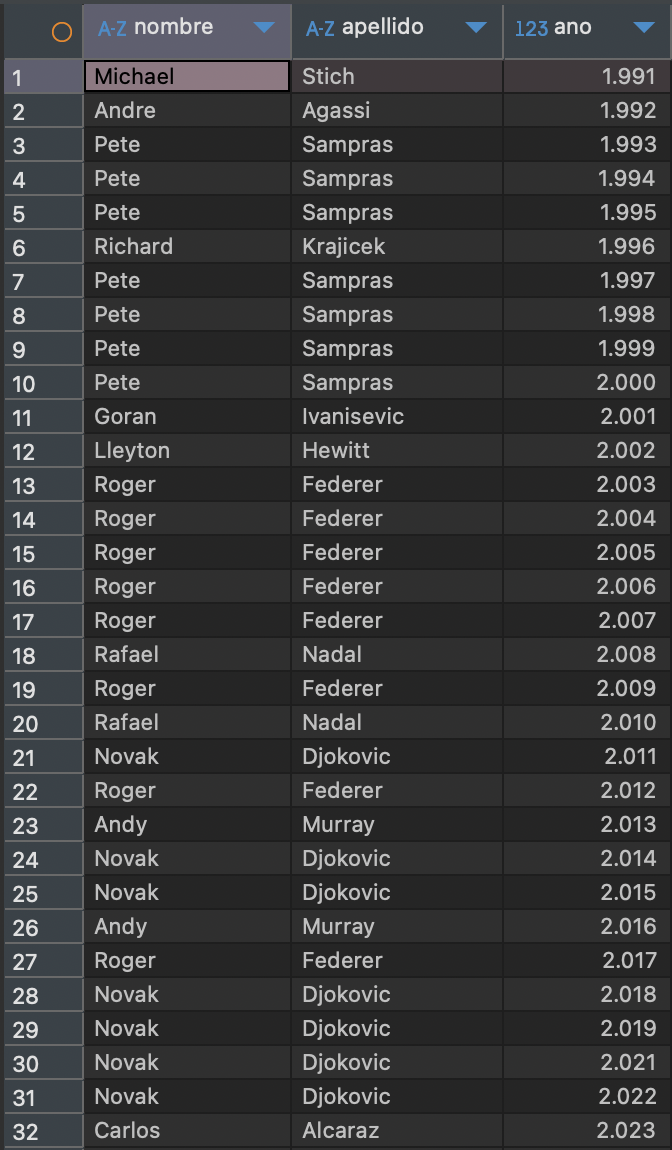
\includegraphics[height=0.4\textheight]{fotos/q1_json.png}
\caption{Datos agregados en SQL. Tipo JSON, consulta 1.}
\label{fig:q1_json}
\end{figure}



\subsubsection{Muestra los años en los que Roger Federer ganó algún torneo de nivel Gran Slam (G) o Master 1000 (M). Para cada año, muestra el número de torneos y lista sus nombres (ordenados por la fecha de celebración). Ordena el resultado por el año}

Para esta consulta partimos del mismo punto que para la anterior: el producto cartesiano de la tabla \texttt{tenisjson} con la función \texttt{jsonb\_array\_elements(partidos\_ganados)}. Esta vez, la selección es más específica: queremos los partidos finales (accedemos en \texttt{ronda} como texto) de torneos Grand Slam o Master 1000 (accedemos como texto con \texttt{`torneo'} ->> \texttt{`nivel'}), donde el ganador sea Roger Federer (accedemos al nombre y apellido como texto del jugador desde \texttt{jugador}). Esto nos da una tupla para cada final ganada por Federer, por lo que para nuestro resultado debemos hacer un \texttt{group by} por año. Así, tenemos una tupla para cada año. \\

Finalmente, obtenemos la proyección usando el año del torneo (al cual accedemos como en la anterior consulta), el conteo de los torneos (usamos \texttt{count(distinct)} sobre el nombre de los torneos para evitar contar repetidos) y los nombres de los torneos (usamos \texttt{string\_agg} para concatenar los nombres de los torneos, ordenados por fecha de celebración). Ordenamos el resultado final por año en orden ascendente. La consulta se muestra a continuación, y el resultado es el esperado (figura \ref{fig:q2_json})

\begin{minted}[frame=single, fontsize=\footnotesize]{sql}
select extract(year from (pg -> 'torneo' ->> 'fecha')::date) as ano,
    count(distinct pg -> 'torneo'->>'nombre') as numero_torneos,
    string_agg(pg -> 'torneo'->>'nombre', ', ' order by pg -> 'torneo' ->> 'fecha') as torneos
from tenisjson tj, jsonb_array_elements(partidos_ganados) as partidos(pg)
where tj.jugador ->> 'nombre' = 'Roger'
    and tj.jugador ->> 'apellido' = 'Federer'
    and pg ->> 'ronda' = 'F'
    and pg -> 'torneo'->>'nivel' in ('G', 'M')
group by ano
order by ano
\end{minted}

\begin{figure}[H]
\centering
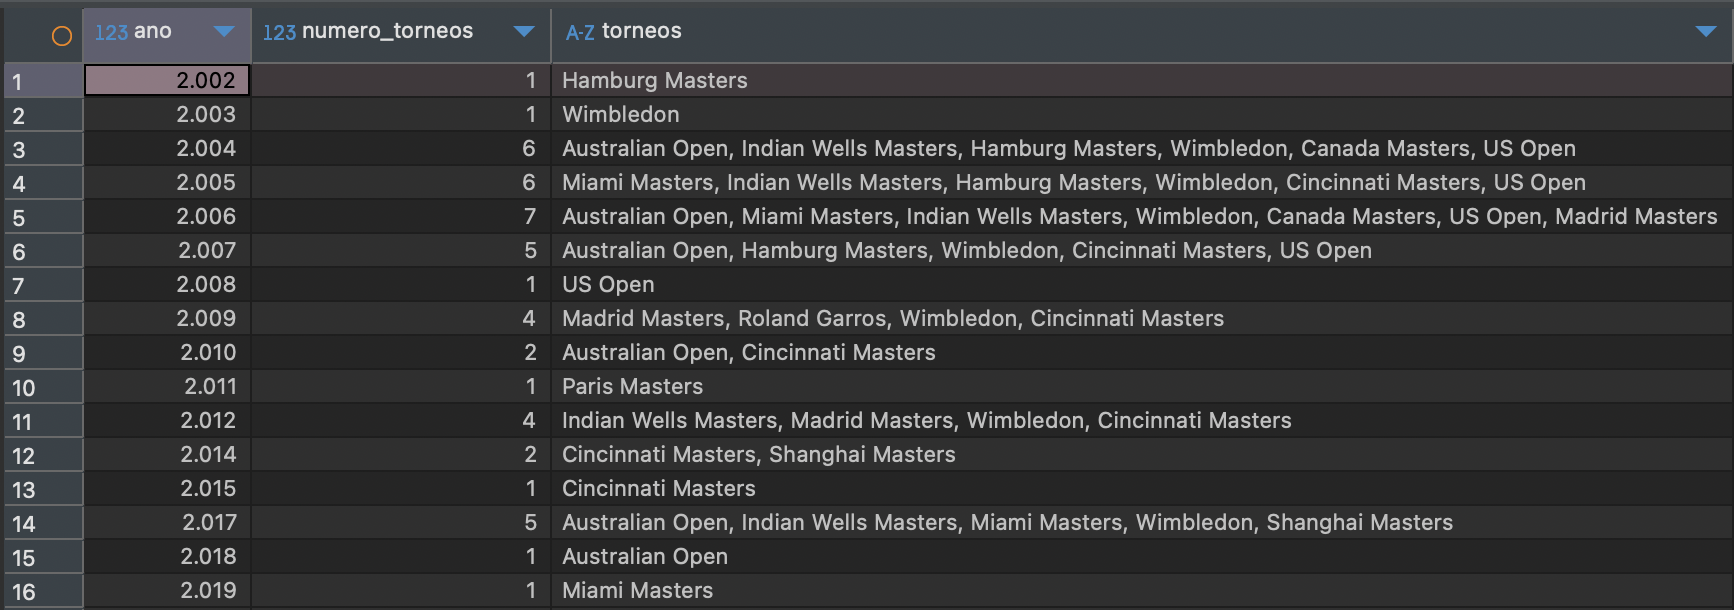
\includegraphics[width=0.8\textwidth]{fotos/q2_json.png}
\caption{Datos agregados en SQL. Tipo JSON, consulta 2.}
\label{fig:q2_json}
\end{figure}



\subsubsection{Muestra los partidos de semifinales (ronda='SF') y final (ronda = 'F') del torneo de "Roland Garros" del 2018. Para cada partido muestra la ronda, el tipo de desenlace, el nombre y apellidos del ganador y el nombre y apellidos del perdedor y el resultado con el número de juegos del ganador y del perdedor en cada set, y opcionalmente en paréntesis el número de juegos del perdedor en el tie break}

Para esta consulta, partimos del producto cartesiano de la tabla \texttt{tenisjson} con las funciones \texttt{jsonb\_array\_el-}\\\texttt{ements(partidos\_ganados)} y \texttt{jsonb\_array\_elements(pg} -> \texttt{`sets')} para extraer los elementos jsonb de partidos ganados y extraer los elementos del objeto jsonb `sets', que designaremos por un alias. Esta vez estamos considerando dos veces la tabla \texttt{tenisjson}, ya que necesitamos estadísticas del ganador y del perdedor. Con esto tenemos de nuevo un exceso de filas debido al producto cartesiano, por lo que seleccionamos los partidos de semifinales y finales de Roland Garros 2018 (accedemos a la ronda, la fecha y al nombre del torneo como texto). Además, seleccionamos solo las tuplas donde el \texttt{id} del jugador rival coincida con el \texttt{id} del jugador de la segunda tabla \texttt{tenisjson} que consideramos. Con todo esto, tenemos una tupla para cada set de cada partido de semifinales y finales de Roland Garros 2018. Como esto no es lo que queremos, agrupamos por \texttt{ronda}, \texttt{desenlace} y nombre y apellidos del ganador y del perdedor. \\

Con todo esto tenemos simplemente una tupla por cada partido (3, 2 para semifinales y una para final). Para la proyección, seleccionamos la ronda, el desenlace, el nombre y apellidos del ganador y del perdedor como texto (nótese que al concatenar nombre y apellidos debemos hacer la conversión explícita de los atributos a texto) y el resultado, que se construye concatenando el número de juegos del ganador y del perdedor en cada set, y opcionalmente el número de juegos del perdedor en el tie break (si este existe). La consulta se muestra a continuación, y el resultado es el esperado (figura \ref{fig:q3_json})

\begin{minted}[frame=single, fontsize=\footnotesize]{sql}
select pg ->> 'ronda' as ronda, pg ->> 'desenlace' as desenlace, 
	(tj.jugador ->> 'nombre')::text || ' ' || (tj.jugador ->> 'apellido')::text as ganador, 
	(tjr.jugador ->> 'nombre')::text || ' ' || (tjr.jugador ->> 'apellido')::text as perdedor, 
	string_agg((s ->> 'juegos_ganador')::text || '-' || (s ->> 'juegos_perdedor')::text || 
		case when s ->> 'puntos_tiebreak_perdedor' is not null 
			then '(' || (s ->> 'puntos_tiebreak_perdedor')::text || ')' 
			else '' end, ', ' order by s ->> 'num_set') as resultado
from tenisjson tj, jsonb_array_elements(tj.partidos_ganados) as partidos(pg), 
	jsonb_array_elements(pg -> 'sets') as setss(s), tenisjson tjr
where pg ->'torneo' ->> 'nombre' = 'Roland Garros'
    and extract(year from (pg ->> 'fecha')::date) = 2018
    and pg ->> 'ronda' in ('SF', 'F')
    and tjr.jugador->>'id' = pg ->> 'rival'
group by pg ->> 'ronda', pg ->> 'desenlace', 
	tj.jugador ->> 'nombre', tj.jugador ->> 'apellido', 
	tjr.jugador ->> 'nombre', tjr.jugador ->> 'apellido'
\end{minted}

\begin{figure}[H]
\centering
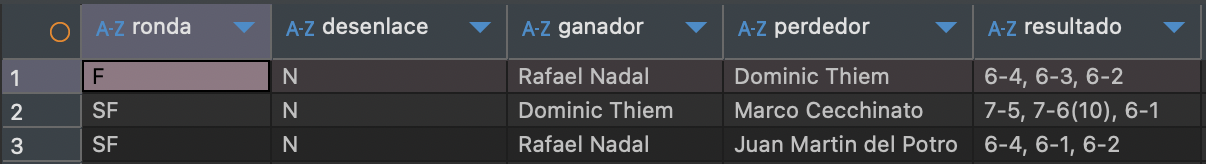
\includegraphics[width=0.7\textwidth]{fotos/q3_json.png}
\caption{Datos agregados en SQL. Tipo JSON, consulta 3.}
\label{fig:q3_json}
\end{figure}



\subsubsection{Muestra la lista de jugadores españoles (ES) que ganaron algún torneo de nivel Gran Slam (G). Para cada jugador muestra los siguientes datos resumen de todos sus partidos: número de partidos jugados, porcentaje de victorias, porcentaje de aces, porcentaje de dobles faltas, porcentaje de servicios ganados, porcentaje de restos ganados, porcentaje de break points salvados (de los sufridos en contra), porcentaje de break points ganados (de los provocados a favor)}


Como anteriormente, se dividirá esta consulta en dos: una primera parte que selecciona los jugadores españoles que ganaron algún torneo de nivel Gran Slam y una segunda parte que calcula los datos resumen de todos sus partidos. \\

Para la primera parte, partimos del producto cartesiano de la tabla \texttt{tenisjson} con la función \texttt{jsonb\_array\_elements(partidos\_ganados)} para extraer los elementos jsonb de partidos ganados. Seleccionamos los jugadores españoles (accedemos al código ISO2 del país como texto) que ganaron algún torneo de nivel Gran Slam (accedemos a la ronda y al nivel del torneo como texto). Con esto, tenemos una tupla para cada partido final ganado por un jugador español en un torneo de nivel Gran Slam. En la proyección, nos quedamos con el \texttt{id} y el nombre y apellido del jugador, usando \texttt{distinct} para evitar duplicados. \\

Para la segunda parte, partimos del producto cartesiano de la tablade jugadores españoles con \texttt{tenisjson} y con la función \texttt{jsonb\_array\_elements(tj.partidos\_ganados)} para extraer los elementos jsonb de partidos ganados. Seleccionamos en el \texttt{where} los partidos en los que los jugadores españoles antes diferenciados aparece, tanto como ganadores como rivales. Con esto, tenemos una tupla para cada partido jugado por un jugador español (que haya ganado un Grand Slam). Antes de hacer la proyección, agrupamos por jugador para tener una tupla para cada jugador. \\

La proyección para obtener las estadísticas del jugador es conceptualmente igual a lo que ya hicimos en esta consulta para el modelo relacional y para el de tipos compuestos. Solo tenemos que tener en cuenta que los valores que queremos están en el objeto jsonb `stats' o en `stats\_rival' de cada partido (es decir, accedemos con ->). Una vez dentro de estos, accedemos con normalidad a las estadísticas que queramos en formato texto con ->>. La consulta se muestra a continuación, y el resultado es el esperado (figura \ref{fig:q4_json})

\begin{minted}[frame=single, fontsize=\footnotesize]{sql}
with jugadores_espanoles_ganadores as (
    select distinct (tj.jugador ->> 'id')::integer as id_jugador, 
    	(tj.jugador ->> 'nombre')::text || ' ' || (tj.jugador ->> 'apellido')::text as jugador
    from tenisjson tj, jsonb_array_elements(partidos_ganados) as partidos(pg)
    where tj.pais ->> 'codigo_iso2' = 'ES'
        and pg ->> 'ronda' = 'F'
        and pg -> 'torneo' ->> 'nivel' = 'G'
)

select jeg.jugador,
    count(*) as partidos,
    round(100.0 * count(case when pg ->> 'rival' = jeg.id_jugador::text then null else 1 end)::numeric / 
	count(*), 1) as pcje_victorias,
    round(100.0 * sum(case when pg ->> 'rival' = jeg.id_jugador::text 
    	then (pg -> 'stats_rival' ->> 'num_aces')::numeric 
    	else (pg -> 'stats' ->> 'num_aces')::numeric end) / 
    	nullif(sum(case when pg ->> 'rival' = jeg.id_jugador::text 
    		then (pg -> 'stats_rival' ->> 'num_puntos_servidos')::numeric 
    		else (pg->'stats'->>'num_puntos_servidos')::numeric end), 0), 1) as pcje_aces,
    round(100.0 * sum(case when pg ->> 'rival' = jeg.id_jugador::text 
    	then (pg -> 'stats_rival' ->> 'num_dob_faltas')::numeric 
    	else (pg -> 'stats' ->> 'num_dob_faltas')::numeric end) / 
    	nullif(sum(case when pg ->> 'rival' = jeg.id_jugador::text 
    		then (pg -> 'stats_rival' ->> 'num_puntos_servidos')::numeric 
    		else (pg -> 'stats' ->> 'num_puntos_servidos')::numeric end), 0), 1) 
			as pcje_dobles_faltas,
    round(100.0 * sum(case when pg ->> 'rival' = jeg.id_jugador::text 
    	then (pg -> 'stats_rival' ->> 'num_primeros_servicios_ganados')::numeric + 
		(pg -> 'stats_rival' ->> 'num_segundos_servicios_ganados')::numeric 
    	else (pg -> 'stats' ->> 'num_primeros_servicios_ganados')::numeric + 
		(pg -> 'stats' ->> 'num_segundos_servicios_ganados')::numeric end) / 
    	nullif(sum(case when pg ->> 'rival' = jeg.id_jugador::text 
    		then (pg -> 'stats_rival' ->> 'num_puntos_servidos')::numeric 
    		else (pg -> 'stats' ->> 'num_puntos_servidos')::numeric end), 0), 1) 
			as pcje_servicios_ganados,
    round(100.0 * sum(case when pg ->> 'rival' = jeg.id_jugador::text 
    	then (pg -> 'stats' ->> 'num_puntos_servidos')::numeric - 
		(pg -> 'stats' ->> 'num_primeros_servicios_ganados')::numeric - 
    		 (pg -> 'stats' ->> 'num_segundos_servicios_ganados')::numeric 
    	else (pg -> 'stats_rival' ->> 'num_puntos_servidos')::numeric - 
		(pg -> 'stats_rival' ->> 'num_primeros_servicios_ganados')::numeric - 
    		 (pg -> 'stats_rival' ->> 'num_segundos_servicios_ganados')::numeric end) / 	
    	nullif(sum(case when pg ->> 'rival' = jeg.id_jugador::text 
    		then (pg -> 'stats' ->> 'num_puntos_servidos')::numeric 
    		else (pg -> 'stats_rival' ->> 'num_puntos_servidos')::numeric end), 0), 1) 
			as pcje_restos_ganados,
    round(100.0 * sum(case when pg ->> 'rival' = jeg.id_jugador::text 
    	then (pg->'stats_rival'->>'num_break_salvados')::numeric 
    	else (pg -> 'stats' ->> 'num_break_salvados')::numeric end) / 
    	nullif(sum(case when pg ->> 'rival' = jeg.id_jugador::text 
    		then (pg -> 'stats_rival' ->> 'num_break_afrontados')::numeric 
    		else (pg -> 'stats' ->> 'num_break_afrontados')::numeric end), 0), 1) 
			as pcje_breaks_salvados,
    round(100.0 * sum(case when pg ->> 'rival' = jeg.id_jugador::text 
    	then (pg -> 'stats' ->> 'num_break_afrontados')::numeric - 
		(pg -> 'stats' ->> 'num_break_salvados')::numeric
    	else (pg -> 'stats_rival' ->> 'num_break_afrontados')::numeric - 
		(pg -> 'stats_rival' ->> 'num_break_salvados')::numeric end) / 
    	nullif(sum(case when pg ->> 'rival' = jeg.id_jugador::text 
    		then (pg -> 'stats' ->> 'num_break_afrontados')::numeric 
    		else (pg -> 'stats_rival' ->> 'num_break_afrontados')::numeric end), 0), 1) 
			as pcje_breaks_ganados
from jugadores_espanoles_ganadores jeg, tenisjson tj, 
	jsonb_array_elements(tj.partidos_ganados) as partidos(pg)
where (tj.jugador ->> 'id')::integer = jeg.id_jugador 
	or pg ->> 'rival' = jeg.id_jugador::text
group by jeg.jugador
\end{minted}


\begin{figure}[H]
\centering
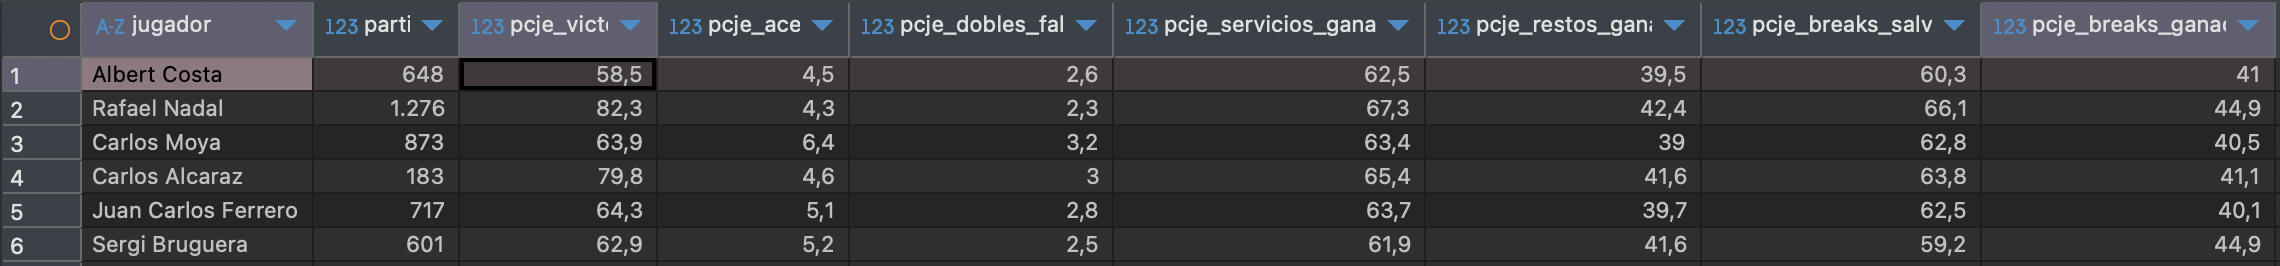
\includegraphics[width=\textwidth]{fotos/q4_json.png}
\caption{Datos agregados en SQL. Tipo JSON, consulta 4.}
\label{fig:q4_json}
\end{figure}


\subsubsection{Lista los jugadores que fueron derrotados (en algún partido del 2018) por el rival de Rafael Nadal de la primera ronda (R128) de Roland Garros de 2018}

Esta consulta la dividiremos en dos subconsultas: una que selecciona el rival de Rafael Nadal en la primera ronda de Roland Garros 2018 y otra que selecciona los jugadores que fueron derrotados por este rival en algún partido del 2018. \\

Para la primera parte, partimos del producto cartesiano de la tabla \texttt{tenisjson} (por duplicado, para discernir entre ganador y perdedor) con la función \texttt{jsonb\_array\_elements(partidos\_ganados)} para extraer los elementos jsonb de partidos ganados. Seleccionamos solo las tuplas que nos interesan: 
\begin{itemize}
\item El nombre torneo debe ser Roland Garros.
\item La ronda debe ser R128.
\item El año de la fecha debe ser del 2018.
\item El nombre y apellido de un jugador debe ser Rafael Nadal, respectivamente. Como no sabemos si ganó o perdió, debemos considerar ambos casos: si es ganador (buscando en la tabla \texttt{tenisjson tj}), o si es perdedor (buscando en la tabla \texttt{tenisjson} con el alias \texttt{tjr}).
\end{itemize}

Con esto, tenemos un única tupla con el rival de Rafael Nadal en la primera ronda de Roland Garros 2018. Proyectamos para obtener el \texttt{id} del jugador rival y el nombre y apellido del jugador, considerando que, cuando el ganador sea Nadal, debemos obtener el rival desde \texttt{tjr}, mientras que en caso contrario, debemos obtener al rival desde \texttt{tj}. No explicamos como acceder a los atributos concretos ya que ya se ha hecho con anterioridad para estos parámetros concretos. El resultado lo guardamos en una tabla temporal \texttt{rival\_nadal}. \\

Para la segunda parte, partimos del producto cartesiano de la tabla anterior con \texttt{tenisjson} y con la función \texttt{jsonb\_array\_elements(tj.partidos\_perdidos)} para extraer los elementos jsonb de partidos perdidos. En el \texttt{where} hacemos una selección de las tuplas para las cuales el \texttt{id} del rival (es decir, el ganador) figure como el del rival de Nadal que encontramos antes. Además, seleccionamos solo los partidos del 2018. Con esto, tenemos una tupla para cada partido ganado por este jugador en el año 2018 (no hay repetidos). En la proyección, seleccionamos simplemente el nombre y apellido del jugador (que concatenamos al seleccionar como texto con ->>) y el código ISO2 del país. La consulta se muestra a continuación, y el resultado es el esperado (figura \ref{fig:q5_json})

\begin{minted}[frame=single, fontsize=\footnotesize]{sql}
with rival_nadal as (
	select case when tj.jugador ->> 'nombre' = 'Rafael' 
			then (pg ->> 'rival')::integer  
			else (tj.jugador ->> 'id')::integer end as id_jugador,
		case when tj.jugador ->> 'nombre' = 'Rafael' 
			then (tjr.jugador ->> 'nombre')::text || ' ' || (tjr.jugador ->> 'apellido')::text 
			else (tj.jugador ->> 'nombre')::text || ' ' || (tj.jugador ->> 'apellido')::text 
			end as jugador
	from tenisjson tj, jsonb_array_elements(tj.partidos_ganados) as partidos(pg), tenisjson tjr
    where pg -> 'torneo' ->> 'nombre' = 'Roland Garros' 
    	and pg ->> 'ronda' = 'R128'
		and extract(year from (pg ->> 'fecha')::date) = 2018
        and tjr.jugador->>'id' = pg ->> 'rival'
        and ((tj.jugador ->> 'nombre' = 'Rafael' and tj.jugador ->> 'apellido' = 'Nadal') 
        	or (tjr.jugador ->> 'nombre' = 'Rafael' and tjr.jugador ->> 'apellido' = 'Nadal'))
)

select tj.jugador->>'nombre' || ' ' || (tj.jugador->>'apellido')::text as jugador, 
	tj.pais->>'codigo_iso2' as pais
from rival_nadal rn, tenisjson tj, jsonb_array_elements(tj.partidos_perdidos) as partidos(pg)
where rn.id_jugador = (pg->>'rival')::integer 
	and extract(year from (pg->>'fecha')::date) = 2018
\end{minted}

\begin{figure}[H]
\centering
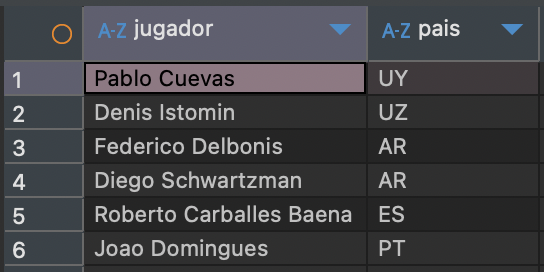
\includegraphics[width=0.35\textwidth]{fotos/q5_json.png}
\caption{Datos agregados en SQL. Tipo JSON, consulta 5.}
\label{fig:q5_json}
\end{figure}
